
%(BEGIN_QUESTION)
% Copyright 2010, Tony R. Kuphaldt, released under the Creative Commons Attribution License (v 1.0)
% This means you may do almost anything with this work of mine, so long as you give me proper credit



\paragraph{Test oppgave Kornsilo lett versjon}

Simulering av kornsiloen ligger i Gand biblioteket. (SimKornsilo)

\begin{tabular}{|c|c|c|c|}
\hline 
Tilkoblet utstyr & IO på RIO & Variabel & Beskrivelse av tilkoblet utstyr\tabularnewline
\hline 
\hline 
Start Knapp & Bryter1 & Start & \tabularnewline
\hline 
Stopp Knapp & Bryter2 & Stopp & \tabularnewline
\hline 
H Sensor & Bryter3 & LevelHigh & \tabularnewline
\hline 
L Sensor & Bryter4 & LevelLow & \tabularnewline
\hline 
Drifts Lys & Lys1 & Drift & \tabularnewline
\hline 
Pumpe Lys & Lys2 & Pumpe & \tabularnewline
\hline 
Alarm Lys & Lys3 & AlarmLys & \tabularnewline
\hline 
Alarm Lyd & Lys4 & AlarmLyd & \tabularnewline
\hline 
\end{tabular}

En kornsilo skal fyllest ved hjelp av en pumpe

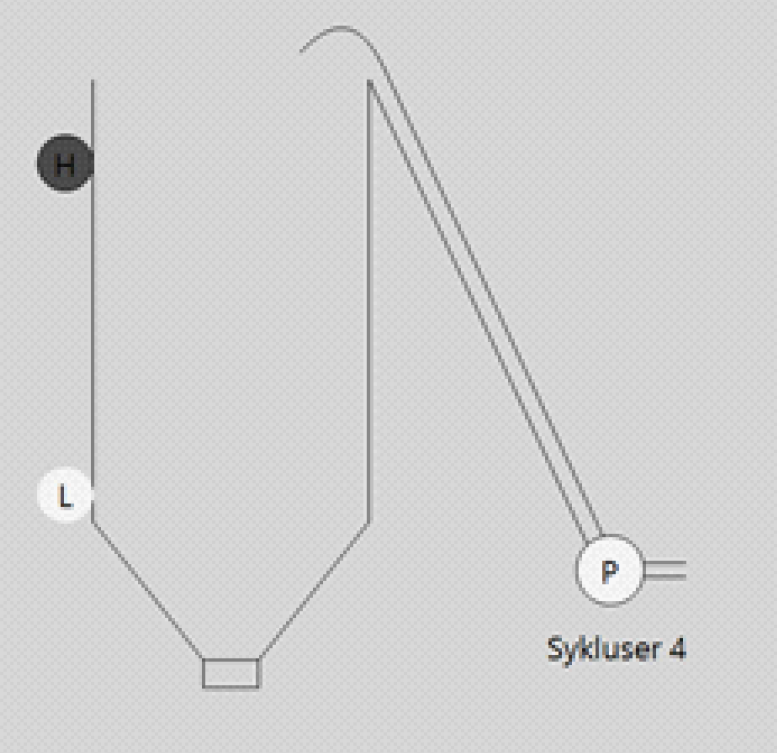
\includegraphics[width=0.5\textwidth]{i08012x01.png}

Der er to nivåvakter i hver silo (L og H) disse gir \textquotedblright{}
TRUE\textquotedblright{} når nivået ligger over giveren.

Virkemåte: Pumpa i en silo skal alltid starte når nivået er under
minimum og stoppe når nivået går over maksimum for siloen.
\begin{enumerate}
\item Lag en Visualisering som ligner den på bildet
\item Anlegget settes i drift med en Start knapp og stoppes med en Stoppknapp.
Når anlegget er satt i drift og nivået er under L startes pumpe P.
Denne går til nivået når H. Slik fortsetter det til driften av anlegget
stoppes.
\item Legg til AutoMan styring av pumpe
\item Legg til en teller for totalt antall sykluser på pumpe (skal vises
på skjerm). 
\item Det skal aktiveres en alarm om det tar mer en 10min (10s) å komme
over L nivå (etter at den har vært under). Alarmen skal ha bekreft
og resett funksjon.
\end{enumerate}

\paragraph{Test oppgave kornsile vanskelig versjon}

Tre kornsiloer skal fyllest ved hjelp av hver sin pumpe P1, P2 og
P3. 

\begin{table}[]
\begin{centering}
\begin{tabular}{|c|c|c|c|}
\hline 
Tilkoblet utstyr & IO på RIO & Variabel & Beskrivelse av tilkoblet utstyr\tabularnewline
\hline 
\hline 
Start Knapp & Bryter1 & Start & \tabularnewline
\hline 
Stopp Knapp & Bryter2 & Stopp & \tabularnewline
\hline 
H Sensor & Bryter3 & LevelHigh & \tabularnewline
\hline 
L Sensor & Bryter4 & LevelLow & \tabularnewline
\hline 
Drifts Lys & Lys1 & Drift & \tabularnewline
\hline 
Pumpe Lys & Lys2 & Pumpe & \tabularnewline
\hline 
Alarm Lys & Lys3 & AlarmLys & \tabularnewline
\hline 
Alarm Lyd & Lys4 & AlarmLyd & \tabularnewline
\hline 
\end{tabular}
\par\end{centering}
\caption{IO-liste for oppkobling mot Gand RIO-trainer}
\end{table}

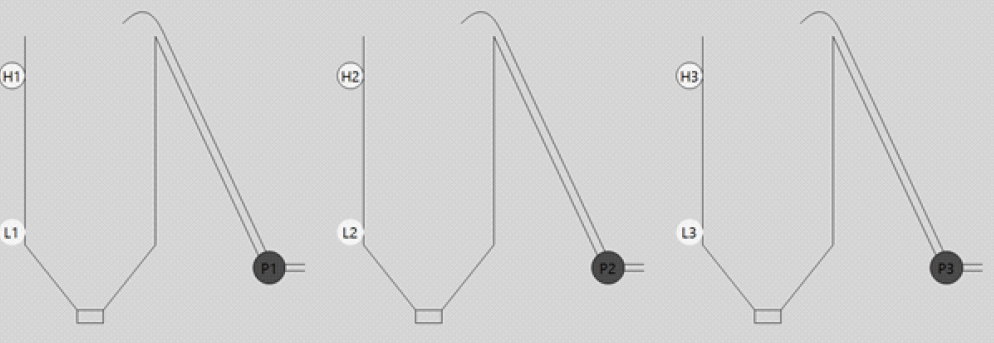
\includegraphics[width=1\textwidth]{i08012x02.png}

Der er to nivåvakter i hver silo (L1, H1, L2. osv.) og alle disse
gir\textquotedblright{} 1\textquotedblright{} når nivået ligger over
giveren. Pumpa i en silo skal alltid starte når nivået er under minimum
og stoppe når nivået går over maksimum for siloen.

Pumpene skal styras slik at det ikke blir brukt mer enn 2000W (P1=500W,
P2=1000W og P3=1500W). Ved tom tank, skal silo fyllest slik at den
ikke lenger er tom (uavhengig av strømforbruk). Alle nettverk programmeres
i LD/FBD. Det skal være mulighet for manuell styring av pumper. 
\begin{enumerate}
\item Anlegget settes i drift med en Start knapp og stoppes med en Stoppknapp.
Når anlegget er satt i drift og nivået er under L startes pumpe P.
Denne går til nivået når H. Dette gjeler for alle pumpene. Slik fortsetter
det til driften av anlegget stoppes. 
\item Komplementer anlegget med alarm dersom nivået ligger under minimum
i mer enn 1 minutt i en av siloene. Alarmsignalet skal pulsere (blinke)
med en frekvens på 1 HZ. 
\item Det er ønskelig med teller for antall sykluser og driftstimer på hver
pumpe. Driftstid og antall sykluser skal presenteres ved hver pumpe.
Når en pumpe kommer over 1000 sykluser eller 1000 driftstimer skal
det vis et varsel om vedlikehold. Dette skal kunne resettes etter
utført vedlikehold. 
\item Sett opp kommunikasjon med Gand-RIO Trainer i henhold til tilordningslisten.
\end{enumerate}
\vskip 10pt
\underbar{file i08012}
%(END_QUESTION)





%(BEGIN_ANSWER)
Det er ikke svar på denne oppgave
%(END_ANSWER)





%(BEGIN_NOTES)


%INDEX% PLC, programming, kombinatorisk 

%(END_NOTES)




